\newpage
\section{Domain Adversarial Training}

\noindent The approach to see if a classifier that was invariant to these domain variations was to train a DANN that appended the CNN model that had been used previously. In order to determine the effectiveness of the DANN in producing a robust network invariant to the domain that the event was produced by, the feature classifier network was measured in the same way that the classifier networks were, and the purity efficiency curves were used to  determine the performance of the network.\medskip

\begin{figure}[t!]
 \centering
 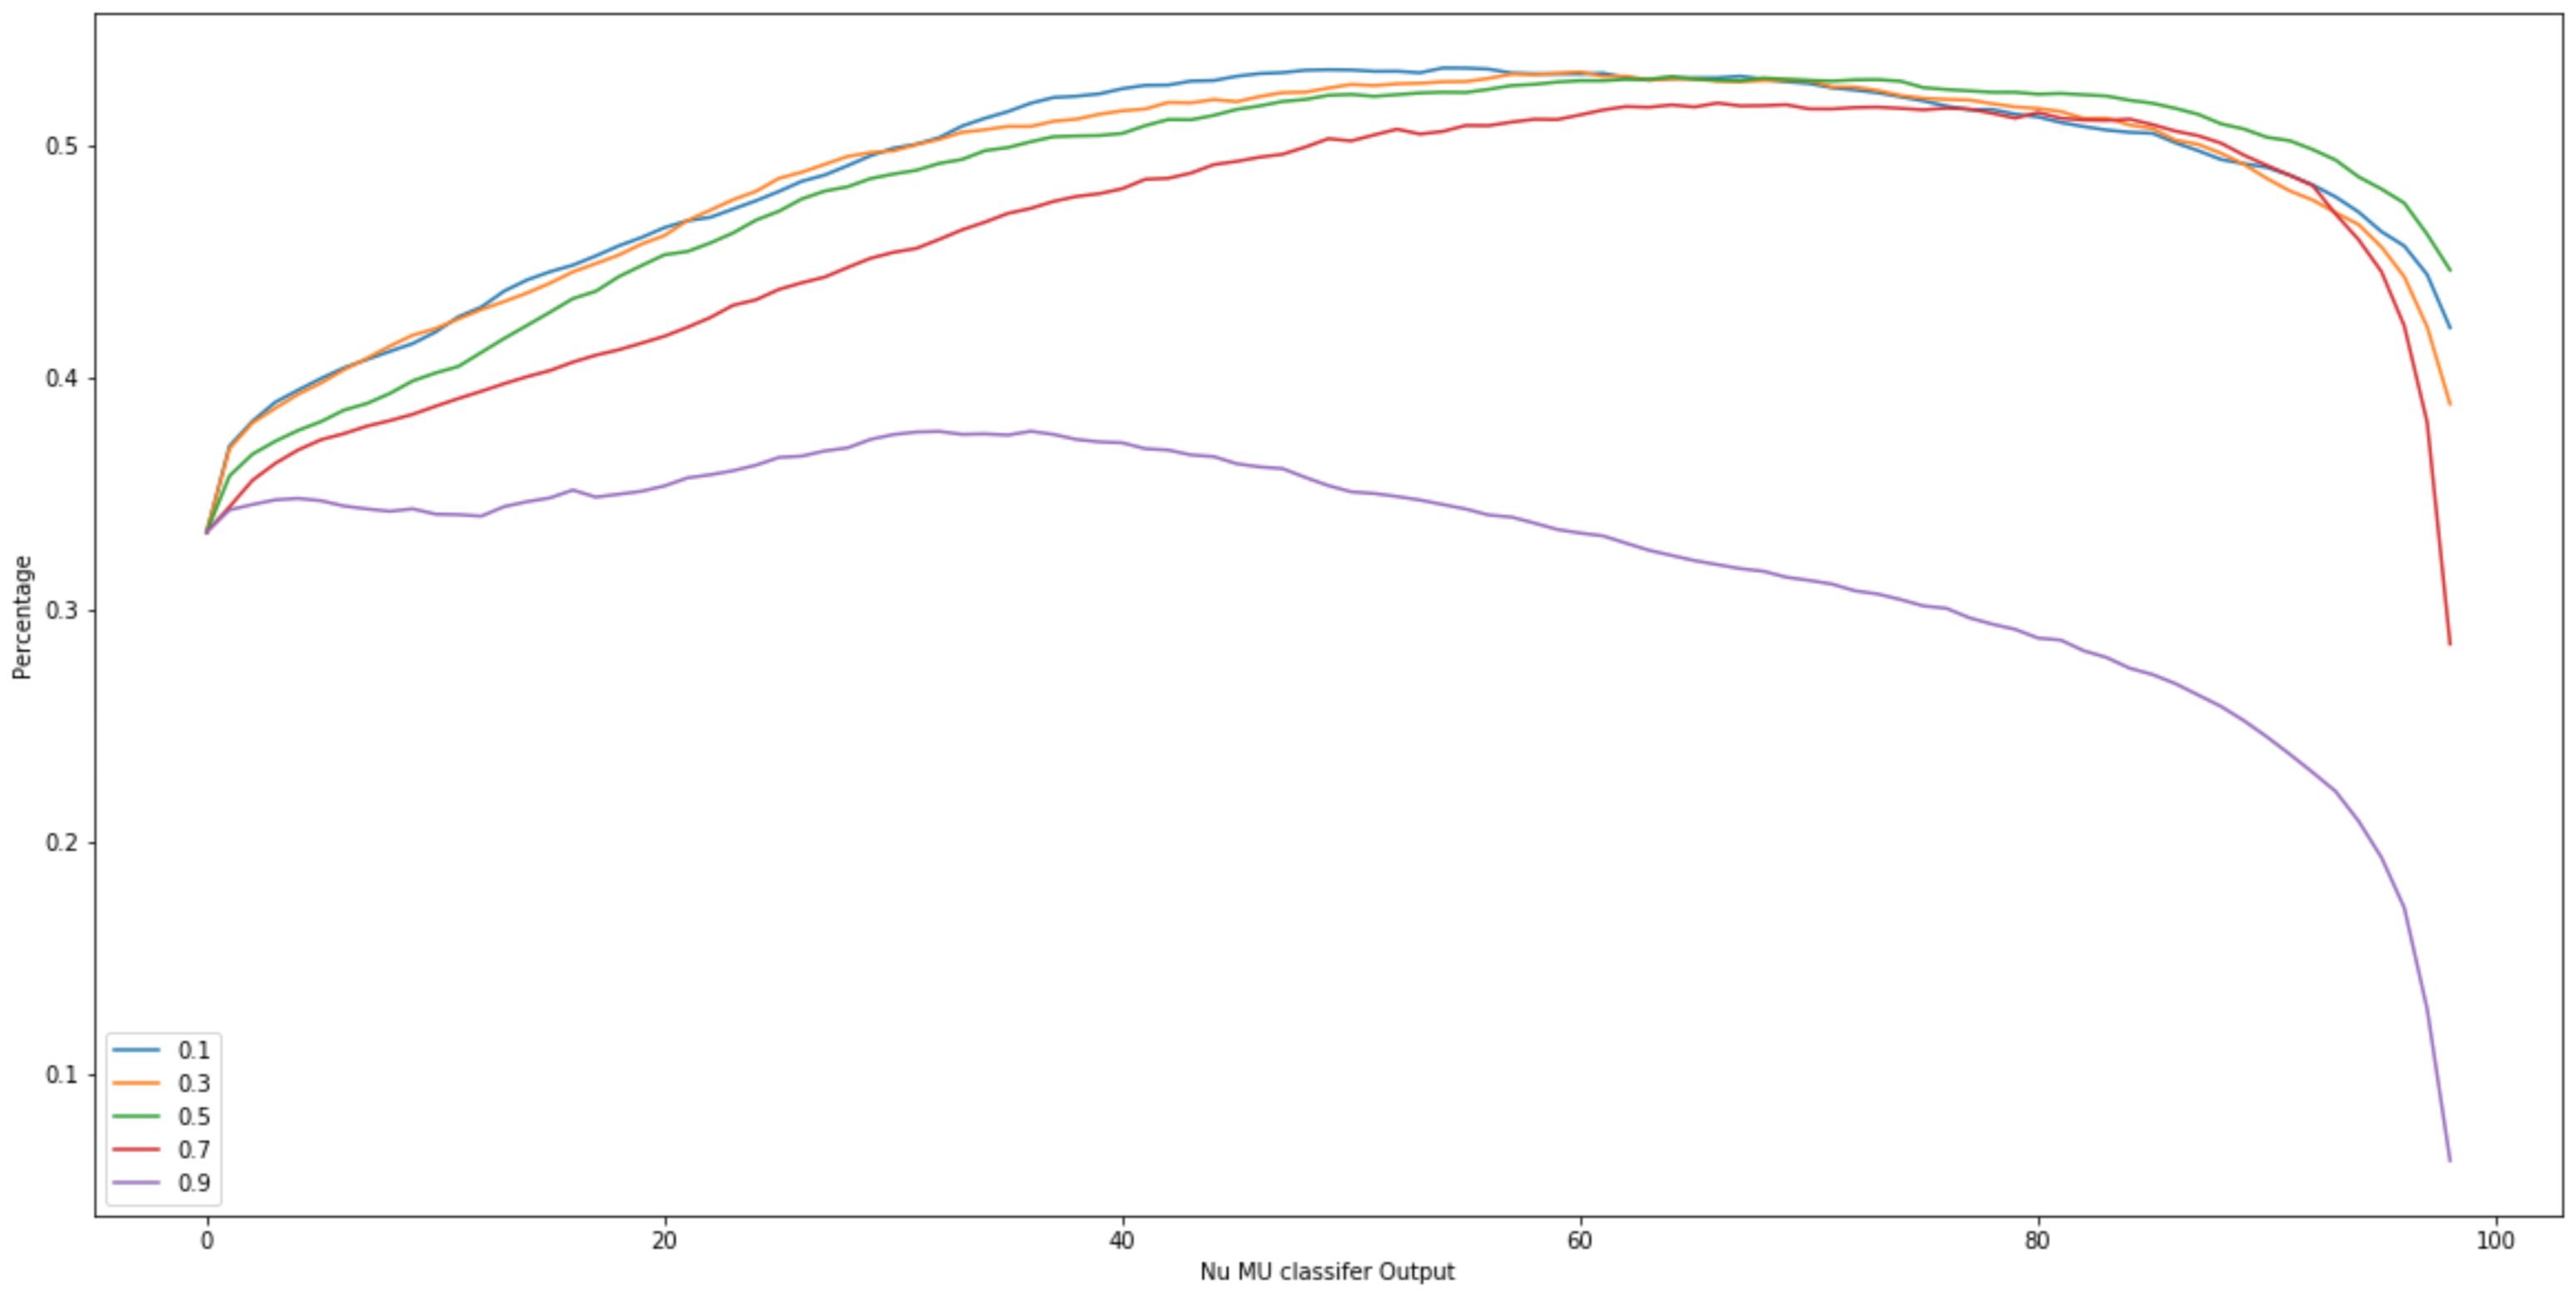
\includegraphics[width=160mm]{dann/dann1.png}
 
 \textbf{Figure 39.} \textit{Purity, efficeny and their product, for DANN $\nu_\mu$ classifier output for DANN gradient reversal scale factors of: 0.1, 0.3, 0.5, 0.7 and 0.9}

 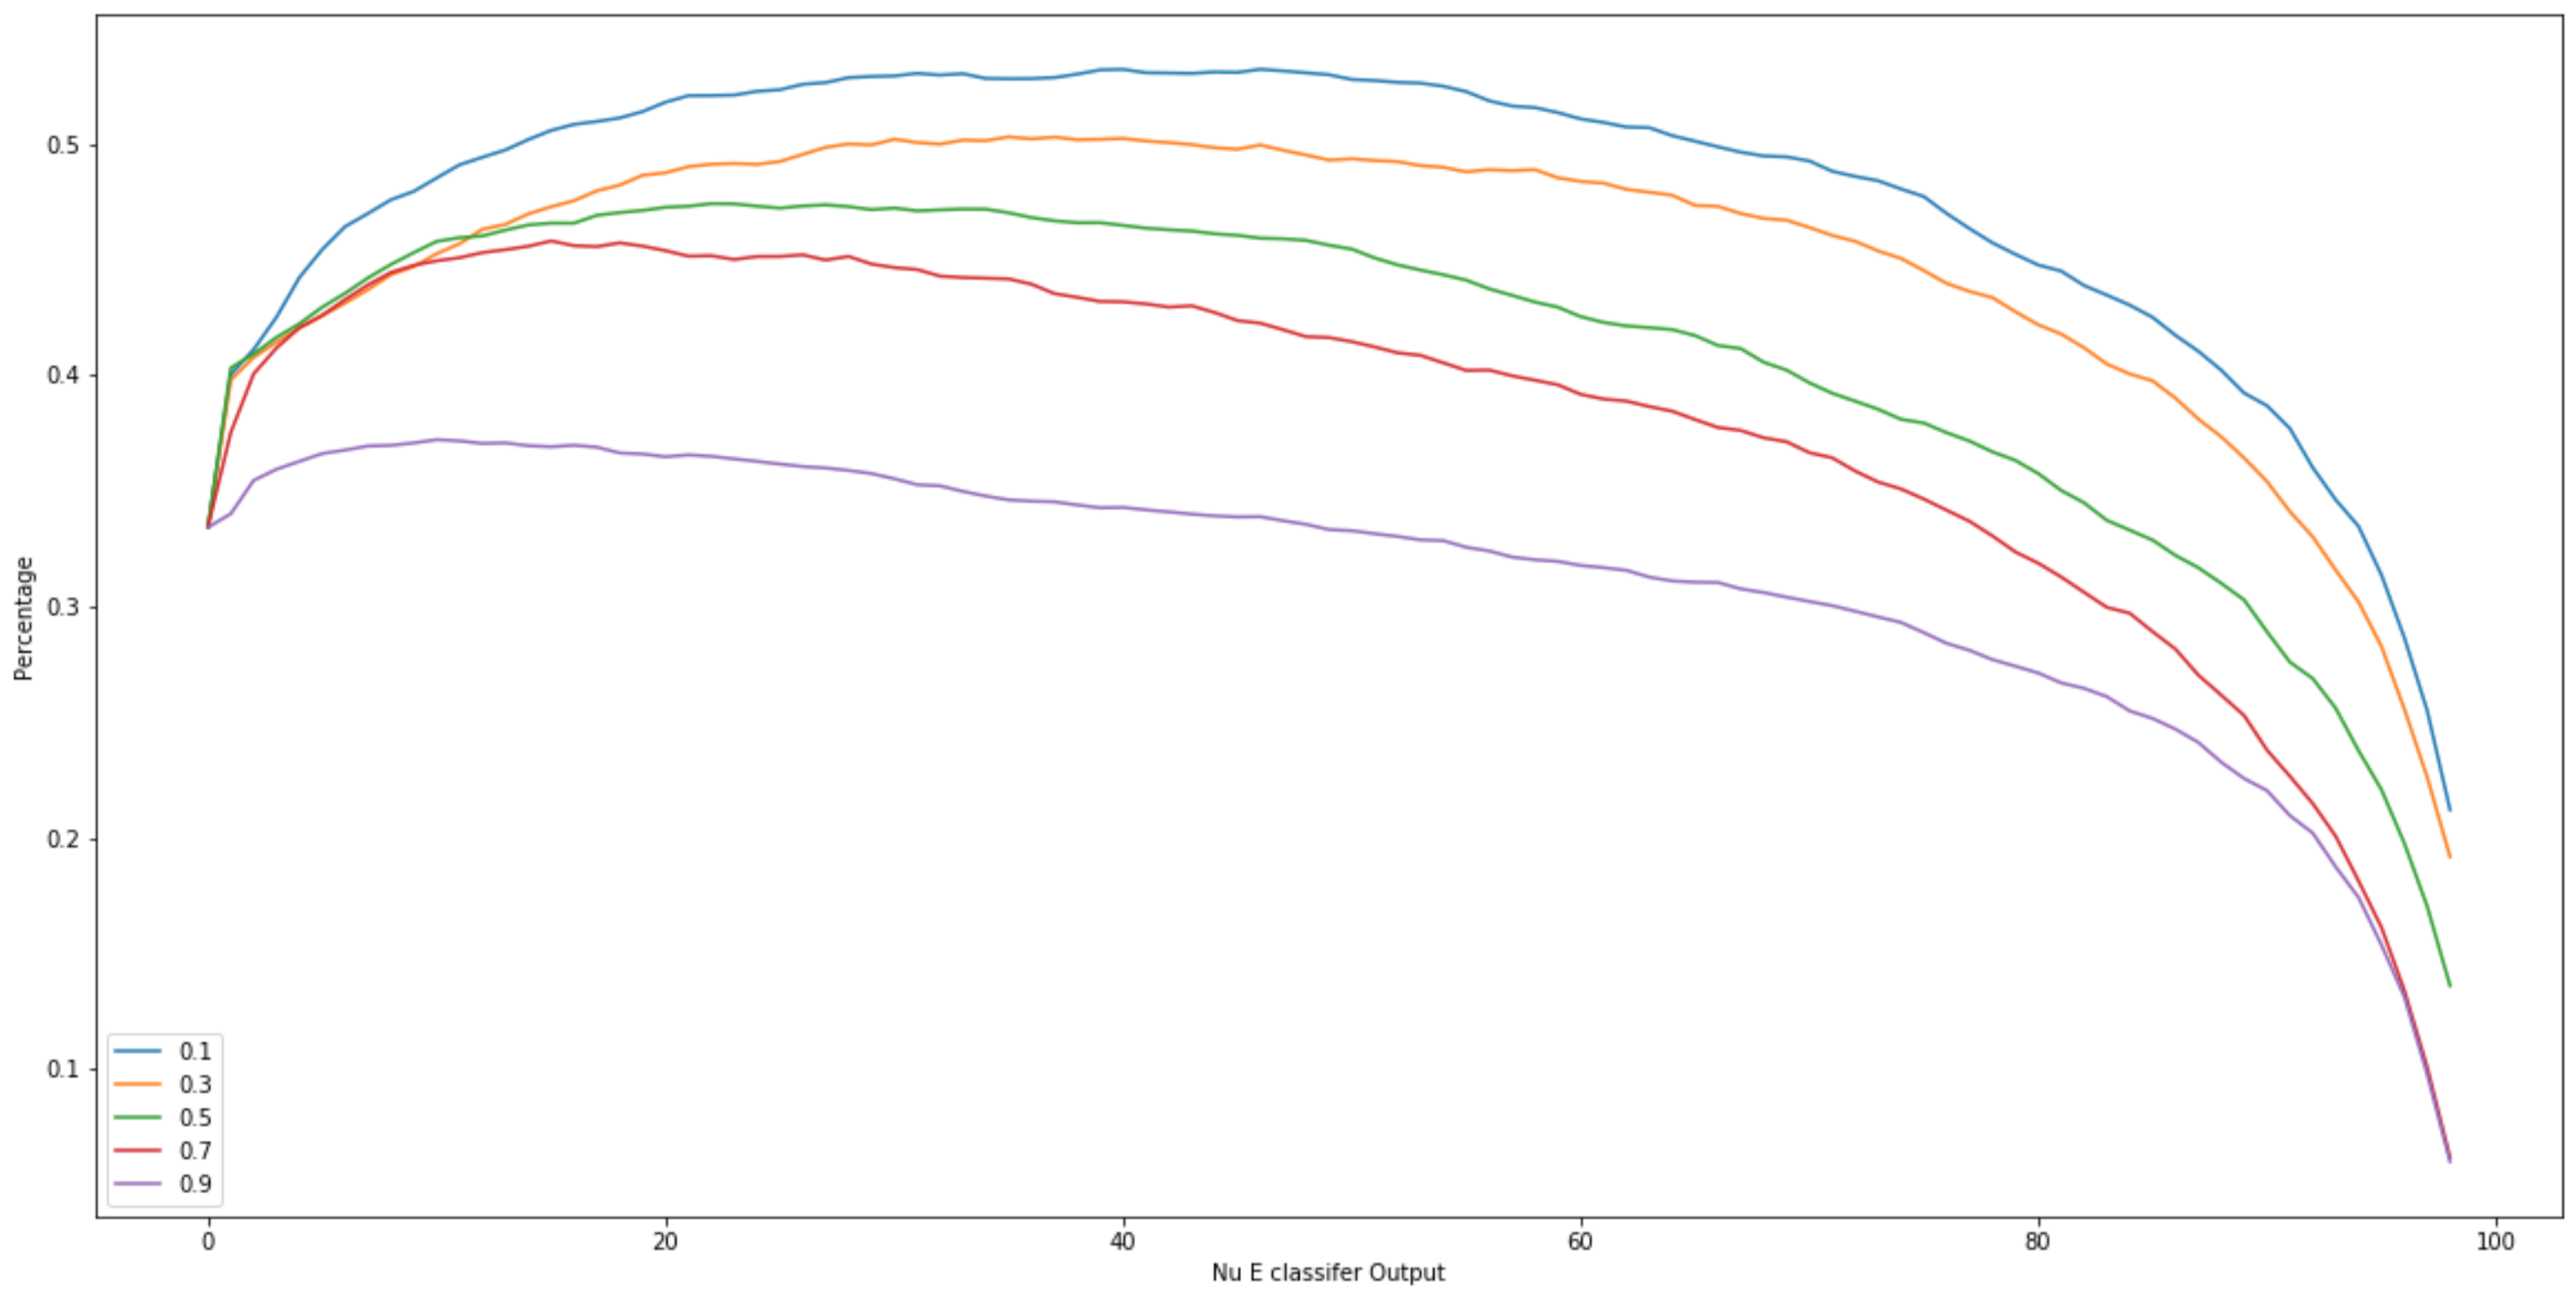
\includegraphics[width=160mm]{dann/dann2.png}
 
 \textbf{Figure 40.} \textit{Purity, efficeny and their product, for DANN $\nu_e$ classifier output for DANN gradient reversal scale factors of: 0.1, 0.3, 0.5, 0.7 and 0.}
\end{figure}

\noindent Scaling factors between 0 and 1, at 0.1, 0.3, 0.5, 0.7 and 0.9, were used in the training process of each model. Again the models were trained, validated and tested on a dataset containing an equal number of each of the three interaction event types, and an equal number of events produced by GiBUU and GENIE. The results of the $\nu_\mu$ classifier are in Figure 39, and show that the performance of the model does reduce as the gradient reversal scaling factor increases. For the smaller values this difference is very small, but as the values increase, the detrimental effect of the gradient reversal has a larger effect on the classification accuracy. This reduction in classification performance can also be seen in the $\nu_e$ classifier in Figure 40. Here the reduction in performance is much larger as the scaling factor increases. \medskip

\noindent This is as expected, in order for the network to become less sensitive to the domain in which the events are being produced, the network is likely to reduce in accuracy as certain events that were easily identified as an interaction type in one of the domains are now being penalised for having such distinctive features. This trade off in classification performance is beneficial however, as the model does not specialise to these distinctive features of the domain, and is better suited to evaluate events from a different domain.\medskip


\noindent In having a more robust model, the difference in classification performance of the model for events from the different domains would tend to zero. This would be as the model performs equally well on events produced by either domain, and thus is invariant to any differences between the two. In Figure 41 a ROC curve is plotted to show the $\nu_\mu$ classification performance for the models of varying gradient scale factors. Different curves were used to plot the performance of events from the two different sources, with solid lines corresponding to GiBUU generated events, and dashed lines for GENIE events, with the colours representing the scale factor used for the training process. While it is very small, it can be seen that the difference in classification performance between the GENIE and GiBUU events does reduce as the scale factor increases. The classification of GENIE events can be seen to increase as the scale factor strength increases, indicating that the model, which previously became overly specialised to GiBUU event features was not less dependent on these which were not found in GENIE events. This does suggest that the $\nu_\mu$ classifier does become more robust as a DANN training process with a larger scale factor takes place- however it is a very small change and would most likely not be considered a negligible improvement when compared to statistical noise. Not all the scale factor training processes were used as the Figure became unreadable, and the scale factor of 0.9 was not used due to it being an exceptionally poor classifier, as seen in Figure 40.\medskip

\begin{figure}[t!]
 \centering
 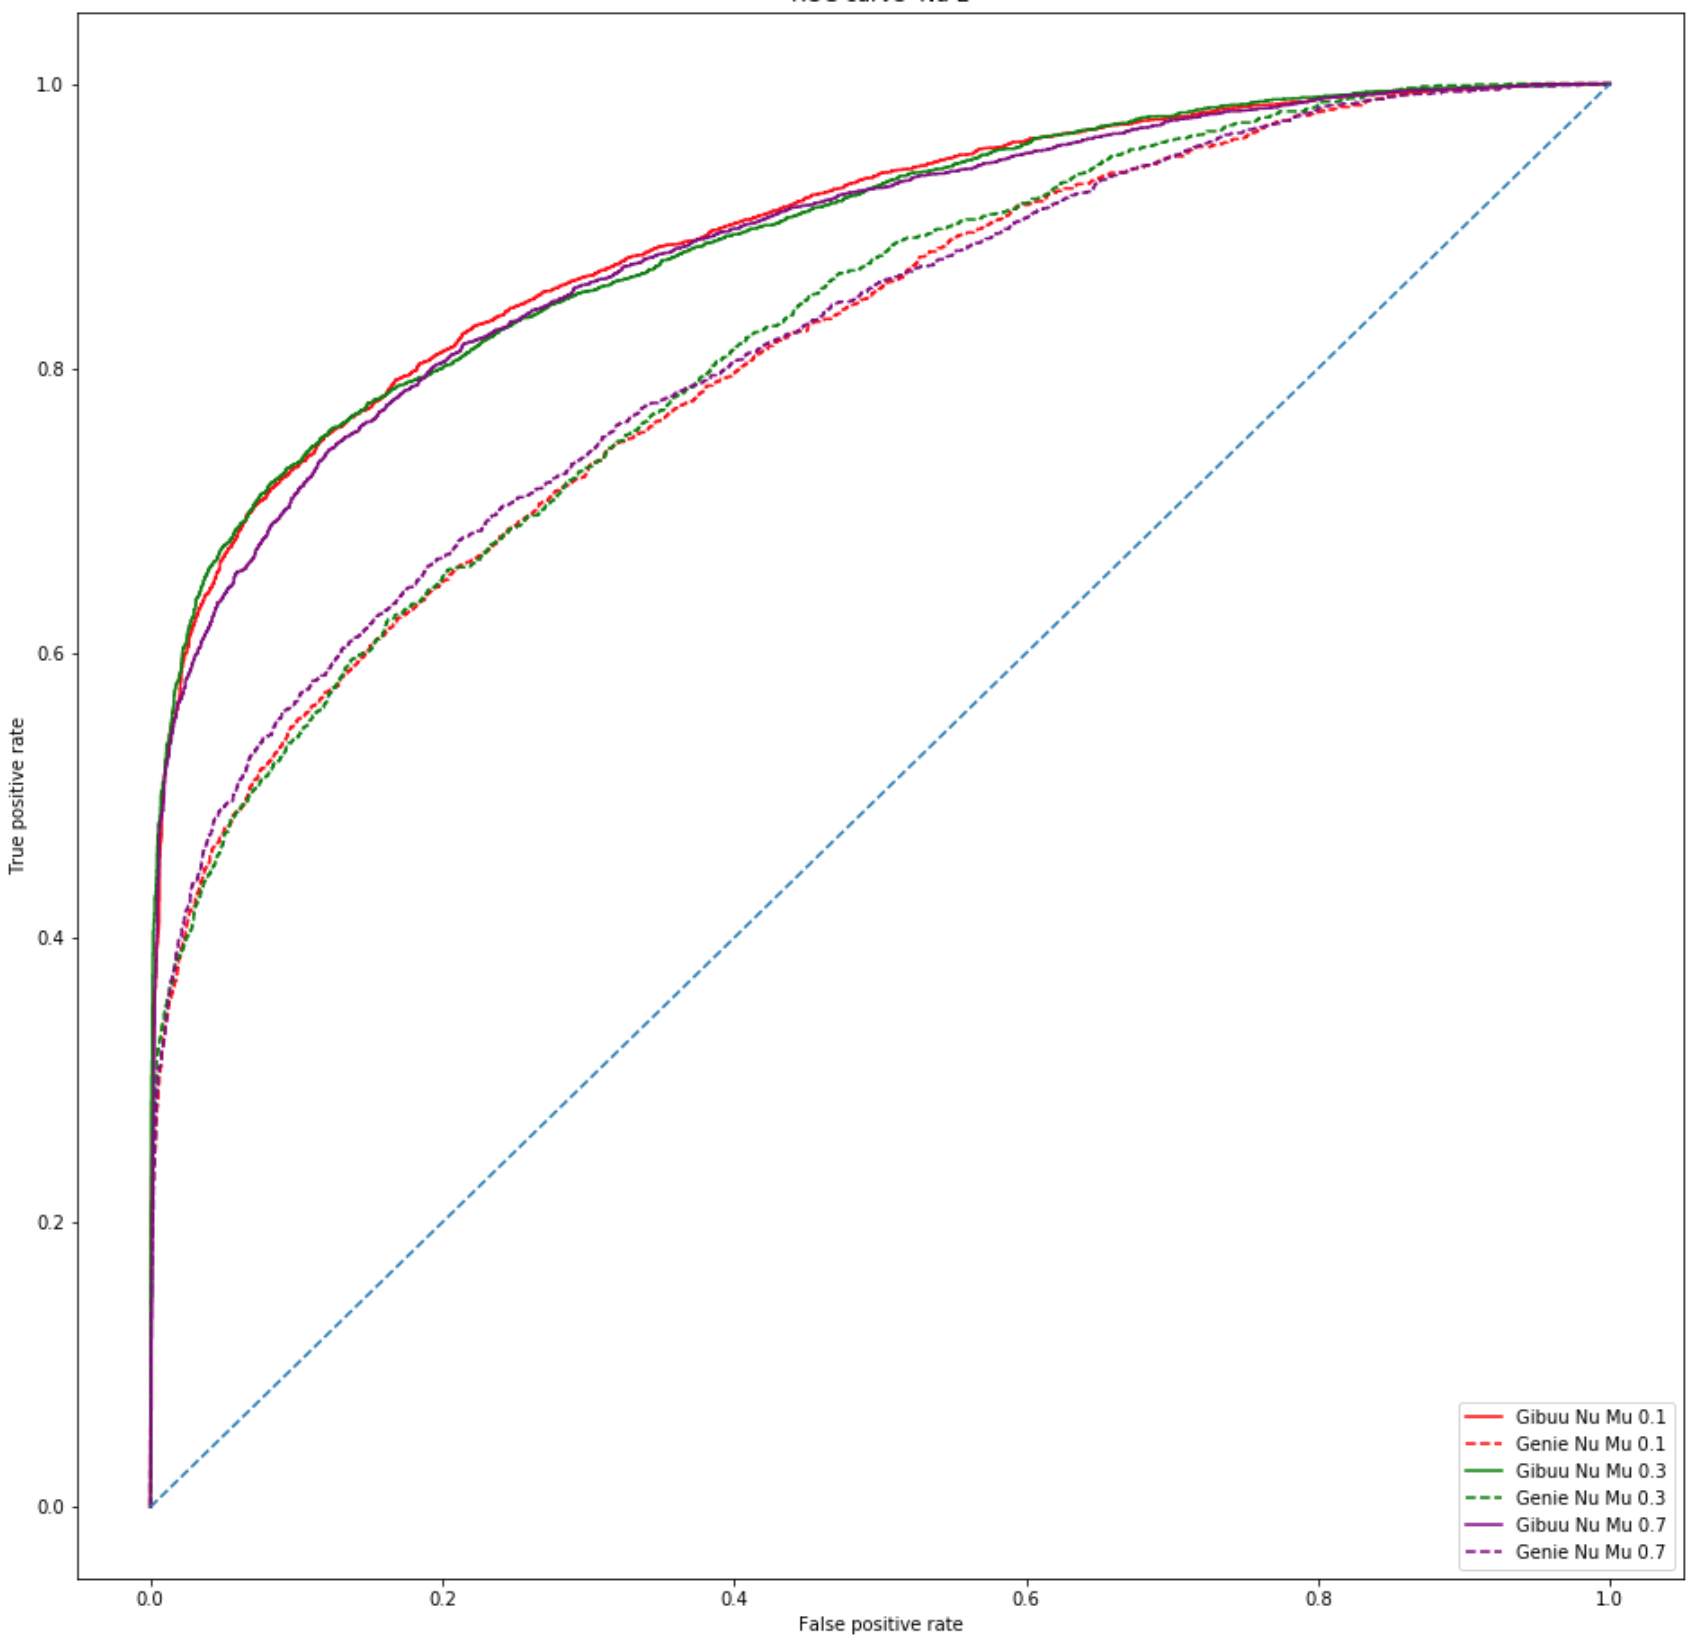
\includegraphics[width=160mm]{dann/dann3.png}
 
 \textbf{Figure 41.} \textit{ROC curve for for DANN $\nu_\mu$ classifier, for DANN gradient reversal scale factors of: 0.1, 0.3, and 0.7, where the GiBUU events are plotted with solid lines and the GENIE curves with dotted lines)}
\end{figure}

\begin{figure}[t!]
 \centering
 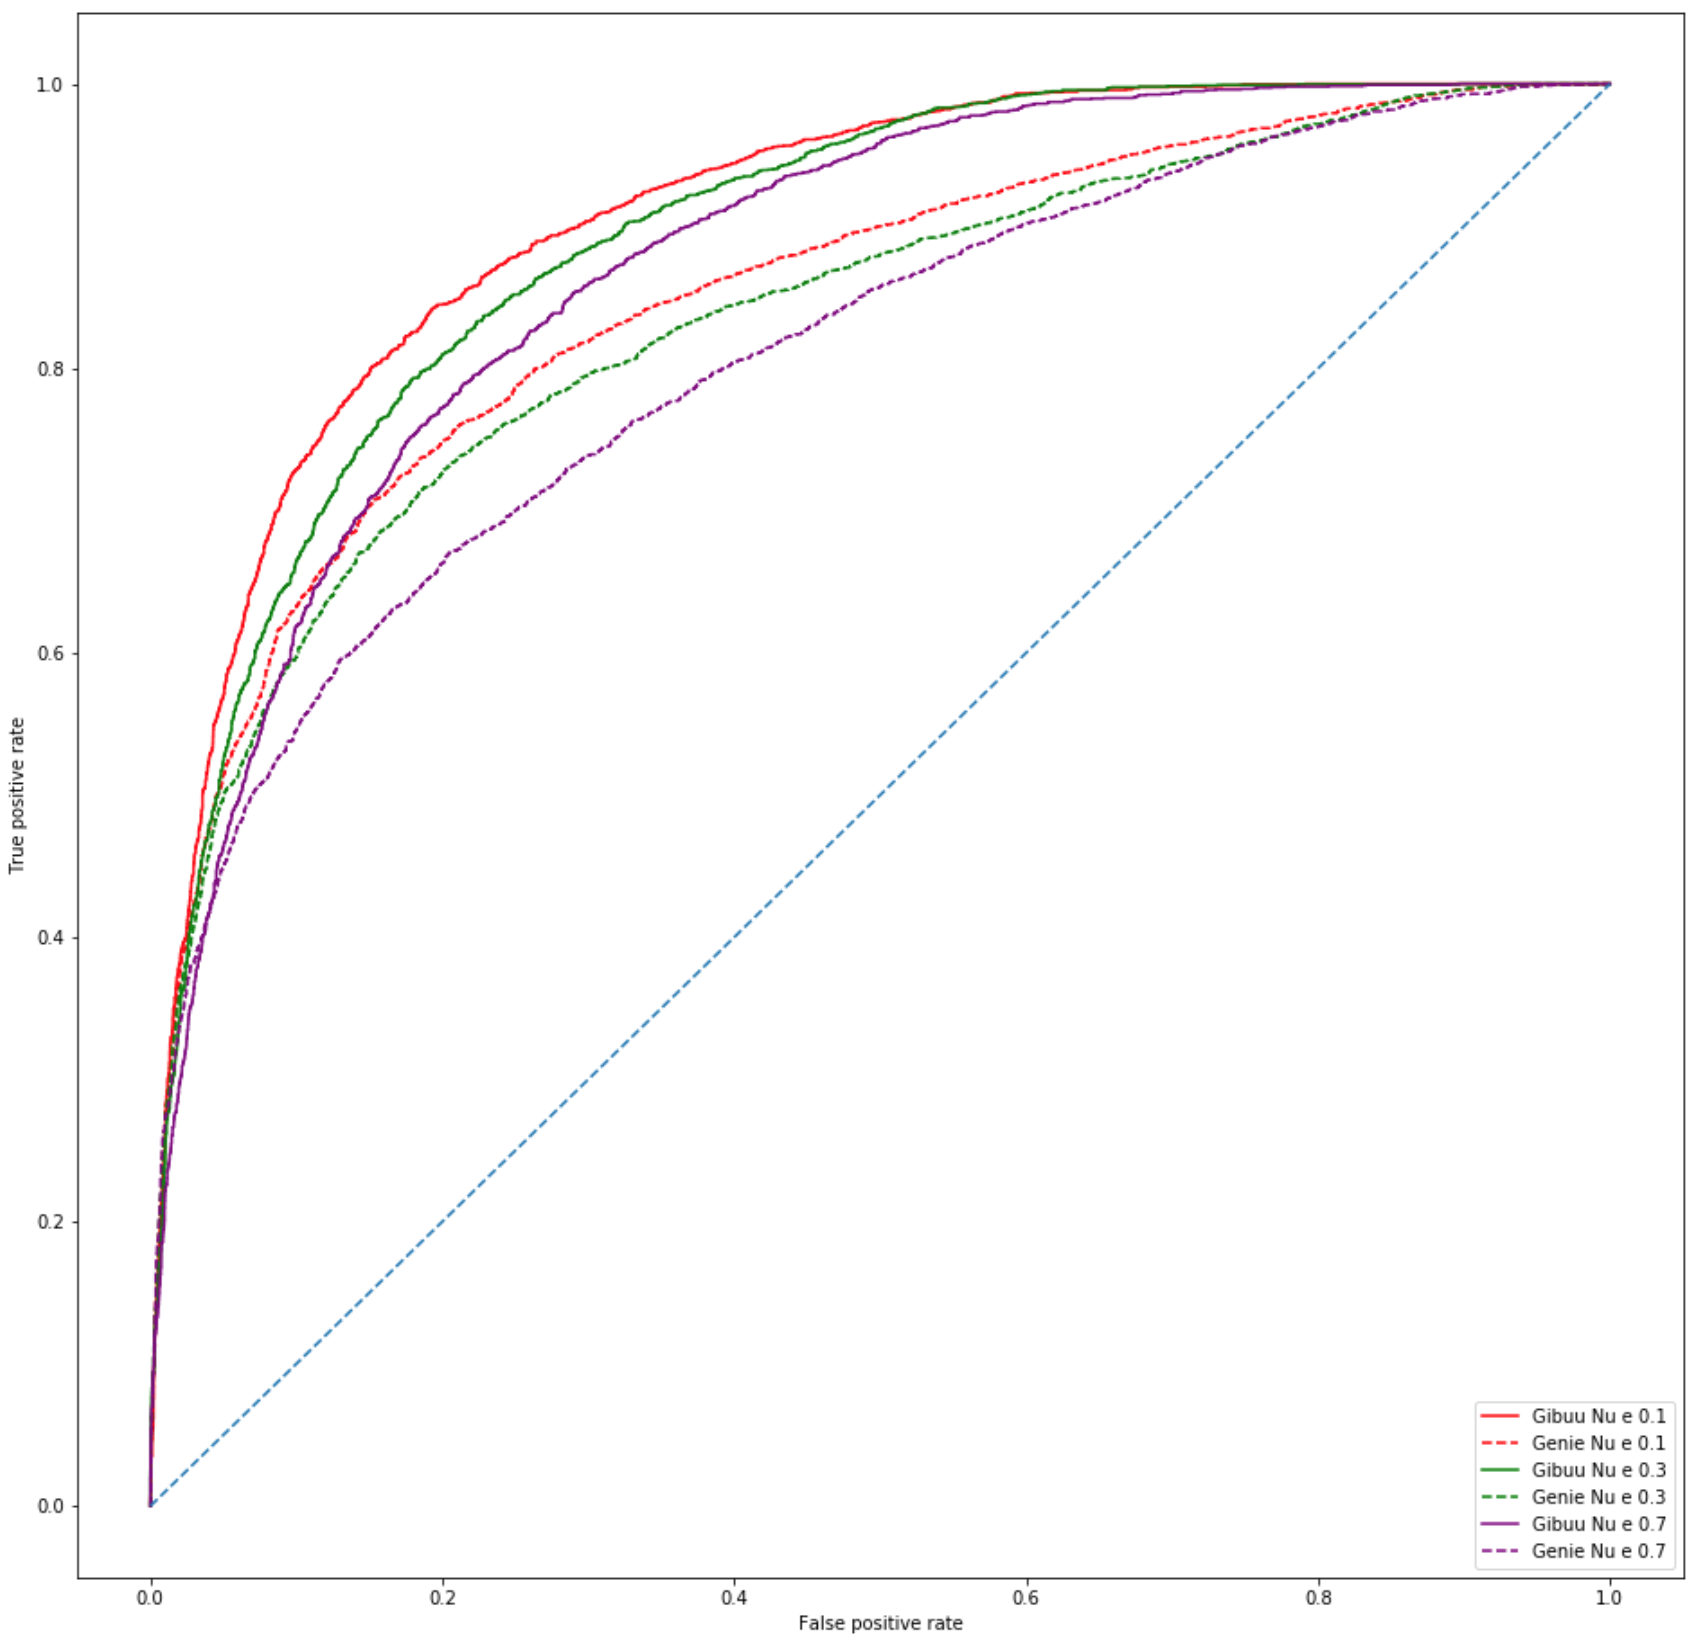
\includegraphics[width=160mm]{dann/dann4.png}
 
 \textbf{Figure 42.} \textit{ROC curve for for DANN $\nu_e$ classifier, for DANN gradient reversal scale factors of: 0.1, 0.3, and 0.7, where the GiBUU events are plotted with solid lines and the GENIE curves with dotted lines}
\end{figure}


\noindent This same increase in robustness cannot be seen by the the $\nu_e$ classifier, Figure 41, where the increase in the strength of the DANN gradient reversal resulted in an overall poorer performance on events produced by both GENIE and GiNUU, with this reduction in performance proportional to the strength of the gradient reversal scale factor. The performance reduces considerably, meaning that the DANN has reduced the network's ability to classify $\nu_e$ events by penalising any ability the network had at discriminating between the two domains. In Figure [], the $\nu_e$ classifier trained on GENIE data performed more poorly when then tested on GiBUU data, indicating that there was a difference the features in the image of a GENIE and GiBUU produced $\nu_e$. The DANN was unable to reduce the difference in classifier performance between events produced from the two domains, suggesting that the $\nu_e$ events now became more difficult to determine now that domain training took place.\medskip


\noindent Figure 36 showed that the nature of the events that were easily identifiable as GiBUU events nearly completely comprised of $NC$ and $\nu_e$ events. The result of successful DANN training would mean that these easily identifiable GiBUU events would result in a negative gradient that backpropagated to make these events less easily identifiable by the network. The proportion of events that were easily identified as being produced by GiBUU that were $\nu_\mu$ events was only 16\%, and thus the DANN process, with regards to these domain identifiable events, was much more limited, which is one reason as to why the DANN process did not reduce the performance of the $\nu_\mu$ classifier. By making the features of these $NC$ and $\nu_e$ events have a reduced impact on the classification process of the network, the network as a result became less successful at identifying these events. \medskip

\noindent This is very straightforward to follow as to how the GiBUU $\nu_e$ performance would have been reduced, but the GENIE performance also fell, leading to a poorer classifier, rather than a more robust one. This may be due to difficulties that are currently the case in classification of GENIE events, such as some $NC$ events looks similar to $\nu_\mu$ events and other similar $\nu_\e$ as displayed in previous sections, but further work would be required to provide insight into this.\medskip



